%%%%%%%%%%%%%%%%%%%%%%%%%%%%%%%%%%%%%%%%%
% Programming/Coding Assignment
% LaTeX Template
%
% This template has been downloaded from:
% http://www.latextemplates.com
%
% Original author:
% Ted Pavlic (http://www.tedpavlic.com)
%
% Note:
% The \lipsum[#] commands throughout this template generate dummy text
% to fill the template out. These commands should all be removed when 
% writing assignment content.
%
% This template uses a Perl script as an example snippet of code, most other
% languages are also usable. Configure them in the "CODE INCLUSION 
% CONFIGURATION" section.
%
%%%%%%%%%%%%%%%%%%%%%%%%%%%%%%%%%%%%%%%%%

%----------------------------------------------------------------------------------------
%	PACKAGES AND OTHER DOCUMENT CONFIGURATIONS
%----------------------------------------------------------------------------------------

\documentclass{article}

\usepackage{fancyhdr} % Required for custom headers
\usepackage{lastpage} % Required to determine the last page for the footer
\usepackage{extramarks} % Required for headers and footers
\usepackage[usenames,dvipsnames]{color} % Required for custom colors
\usepackage{graphicx} % Required to insert images
\usepackage[rightcaption]{sidecap}
\graphicspath{ {images/} }
\usepackage{wrapfig}

\usepackage{listings} % Required for insertion of code
\usepackage{courier} % Required for the courier font
\usepackage{lipsum} % Used for inserting dummy 'Lorem ipsum' text into the template
\usepackage{comment}
\usepackage{amsmath,amsfonts,amsthm}

\lstset{%
   breaklines=true,
   extendedchars=true,
   basicstyle=\ttfamily,
   escapechar=~,
   literate={\→}{$\rightarrow$}1
}

% Margins
\topmargin=-0.45in
\evensidemargin=0in
\oddsidemargin=0in
\textwidth=6.5in
\textheight=9.0in
\headsep=0.25in

\linespread{1.1} % Line spacing

% Set up the header and footer
\pagestyle{fancy}
\lhead{\hmwkAuthorName} % Top left header
\chead{\hmwkClass\ : \hmwkTitle} % Top center head
\rhead{\firstxmark} % Top right header
\lfoot{\lastxmark} % Bottom left footer
\cfoot{} % Bottom center footer
\rfoot{Page\ \thepage\ of\ \protect\pageref{LastPage}} % Bottom right footer
\renewcommand\headrulewidth{0.4pt} % Size of the header rule
\renewcommand\footrulewidth{0.4pt} % Size of the footer rule

\setlength\parindent{0pt} % Removes all indentation from paragraphs

%----------------------------------------------------------------------------------------
%	CODE INCLUSION CONFIGURATION
%----------------------------------------------------------------------------------------

\definecolor{MyDarkGreen}{rgb}{0.0,0.4,0.0} % This is the color used for comments
\lstloadlanguages{sql} % Load Perl syntax for listings, for a list of other languages supported see: ftp://ftp.tex.ac.uk/tex-archive/macros/latex/contrib/listings/listings.pdf
\lstset{language=sql, % Use Perl in this example
        frame=single, % Single frame around code
        basicstyle=\small\ttfamily, % Use small true type font
        keywordstyle=[1]\color{Blue}\bf, % Perl functions bold and blue
        keywordstyle=[2]\color{Purple}, % Perl function arguments purple
        keywordstyle=[3]\color{Blue}\underbar, % Custom functions underlined and blue
        identifierstyle=, % Nothing special about identifiers
        commentstyle=\usefont{T1}{pcr}{m}{sl}\color{MyDarkGreen}\small, % Comments small dark green courier font
        stringstyle=\color{Purple}, % Strings are purple
        showstringspaces=false, % Don't put marks in string spaces
        tabsize=5, % 5 spaces per tab
        %
        % Put standard Perl functions not included in the default language here
        morekeywords={rand},
        %
        % Put Perl function parameters here
        morekeywords=[2]{on, off, interp},
        %
        % Put user defined functions here
        morekeywords=[3]{test},
       	%
        morecomment=[l][\color{Blue}]{...}, % Line continuation (...) like blue comment
        numbers=left, % Line numbers on left
        firstnumber=1, % Line numbers start with line 1
        numberstyle=\tiny\color{Blue}, % Line numbers are blue and small
        stepnumber=5 % Line numbers go in steps of 5
}

% Creates a new command to include a Perl script, the first parameter is the filename of the script (without .pl), the second parameter is the caption
\newcommand{\script}[2]{
\begin{itemize}
\item[]\lstinputlisting[caption=#2,label=#1]{#1}
\end{itemize}
}

%----------------------------------------------------------------------------------------
%	DOCUMENT STRUCTURE COMMANDS
%	Skip this unless you know what you're doing
%----------------------------------------------------------------------------------------

% Header and footer for when a page split occurs within a problem environment
\newcommand{\enterProblemHeader}[1]{
\nobreak\extramarks{#1}{#1 continued on next page\ldots}\nobreak
\nobreak\extramarks{#1 (continued)}{#1 continued on next page\ldots}\nobreak
}

% Header and footer for when a page split occurs between problem environments
\newcommand{\exitProblemHeader}[1]{
\nobreak\extramarks{#1 (continued)}{#1 continued on next page\ldots}\nobreak
\nobreak\extramarks{#1}{}\nobreak
}

\setcounter{secnumdepth}{0} % Removes default section numbers
\newcounter{homeworkProblemCounter} % Creates a counter to keep track of the number of problems

\newcommand{\homeworkProblemName}{}
\newenvironment{homeworkProblem}[1][Problem \arabic{homeworkProblemCounter}]{ % Makes a new environment called homeworkProblem which takes 1 argument (custom name) but the default is "Problem #"
\stepcounter{homeworkProblemCounter} % Increase counter for number of problems
\renewcommand{\homeworkProblemName}{#1} % Assign \homeworkProblemName the name of the problem
\section{\homeworkProblemName} % Make a section in the document with the custom problem count
\enterProblemHeader{\homeworkProblemName} % Header and footer within the environment
}{
\exitProblemHeader{\homeworkProblemName} % Header and footer after the environment
}

\newcommand{\problemAnswer}[1]{ % Defines the problem answer command with the content as the only argument
\noindent\framebox[\columnwidth][c]{\begin{minipage}{0.98\columnwidth}#1\end{minipage}} % Makes the box around the problem answer and puts the content inside
}

\newcommand{\homeworkSectionName}{}
\newenvironment{homeworkSection}[1]{ % New environment for sections within homework problems, takes 1 argument - the name of the section
\renewcommand{\homeworkSectionName}{#1} % Assign \homeworkSectionName to the name of the section from the environment argument
\subsection{\homeworkSectionName} % Make a subsection with the custom name of the subsection
\enterProblemHeader{\homeworkProblemName\ [\homeworkSectionName]} % Header and footer within the environment
}{
\enterProblemHeader{\homeworkProblemName} % Header and footer after the environment
}

%----------------------------------------------------------------------------------------
%	NAME AND CLASS SECTION
%----------------------------------------------------------------------------------------

\newcommand{\hmwkTitle}{Database Project} % Assignment title
%\newcommand{\hmwkDueDate}{} % Due date
\newcommand{\hmwkClass}{CS 340} % Course/class
%\newcommand{\hmwkClassTime}{} % Class/lecture time
%\newcommand{\hmwkClassInstructor}{} % Teacher/lecturer
\newcommand{\hmwkAuthorName}{Chewie Lin (Shuiqiang)} % Your name

%----------------------------------------------------------------------------------------
%	TITLE PAGE
%----------------------------------------------------------------------------------------
\begin{comment}

\title{
\vspace{2in}
\textmd{\textbf{\hmwkClass:\ \hmwkTitle}}\\
\normalsize\vspace{0.1in}\small{Due\ on\ \hmwkDueDate}\\
\vspace{0.1in}\large{\textit{\hmwkClassInstructor\ \hmwkClassTime}}
\vspace{3in}
}

\author{\textbf{\hmwkAuthorName}}
\date{} % Insert date here if you want it to appear below your name

%----------------------------------------------------------------------------------------

\begin{document}

\maketitle

%----------------------------------------------------------------------------------------
%	TABLE OF CONTENTS
%----------------------------------------------------------------------------------------

%\setcounter{tocdepth}{1} % Uncomment this line if you don't want subsections listed in the ToC

\newpage
\tableofcontents
\newpage
\end{comment}

\begin{document}

\homeworkSection{Outline}
This is a database to track the plants grown in one's backyard garden. 
	    There could be many raised beds and hundreds of seeds to track.    
	    I hope it can be used to streamline planting and maximize          
	    productivity of the garden so you can figure out what to plant each
	    month.                                                             
	    You can follow to the link to each of the table to interact with   
	    the database and use the planning page to schedule the garden      
	    plants.


\homeworkSection{Database Outline}

Entities:
\begin{itemize}
	\item Beds - id, name, area
	\item Seeds - id, name, do\_best, sunlight, area, water
	\item Month - id, name, avg\_high, avg\_low, water
	\item Family - id, name, alias
\end{itemize}

Relationship:
\begin{itemize}
	\item many-to-many: seeds can be planted in at least one suitable beds and a bed
		can contain multiple different plants. This can also be used to
		track plants and not plant the same thing in the same bed year
		after year. 
	\item one-to-many: each seed must come from a plant family and a family can
		have multiple seeds. 
	\item one-to-many: each seed is best planted in a specific month but a
		month can be the best time for many plants to grow.
	\item many-to-many: each month affects the sunlight each bed gets over
		the course of the year.
\end{itemize}

\homeworkSection{ER Diagram}
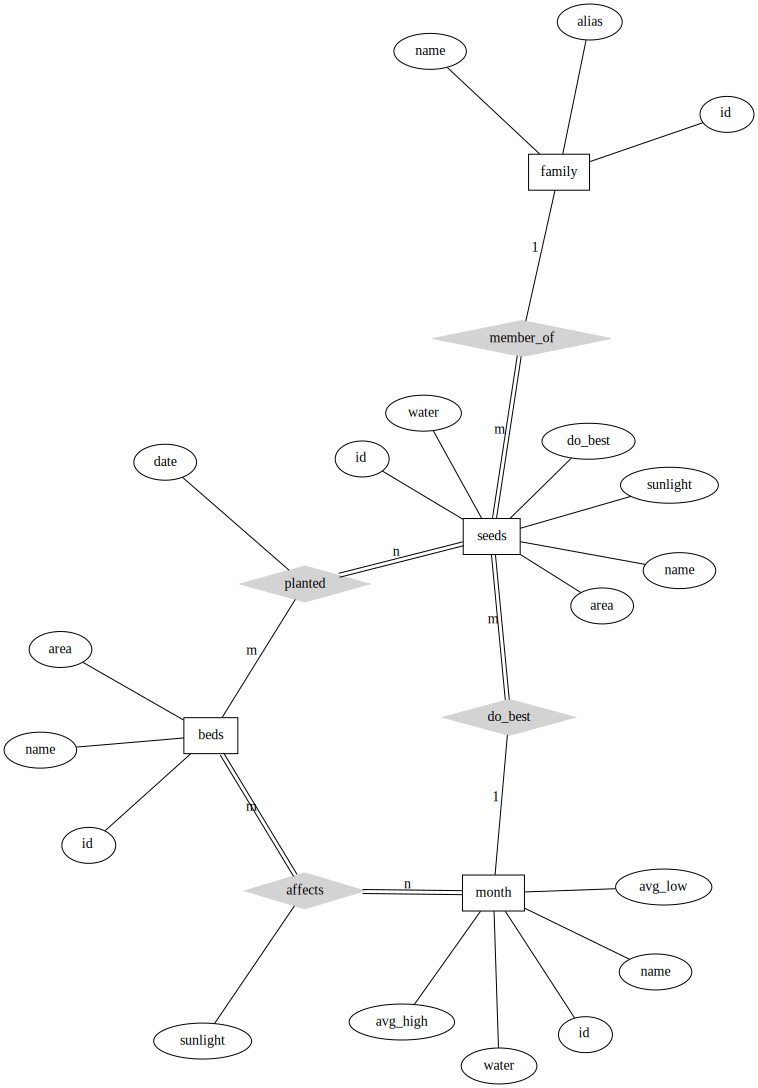
\includegraphics[scale=0.5]{er}


\homeworkSection{Schema}
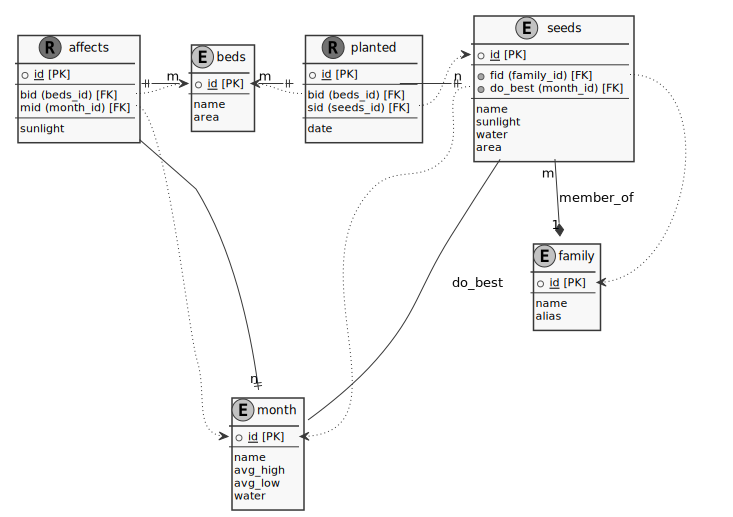
\includegraphics[scale=0.8]{schema}

\homeworkSection{Data Definition Queries}
\lstinputlisting{data_def.sql}

\homeworkSection{Data Manipulation Queries}
\lstinputlisting{data_selection.sql}







\begin{comment}
\homeworkSection{website functionality}
\homeworkSection{style}
\lstinputlisting{debug2.txt}
\lstinputlisting[language={C}]{refactor.txt}
\begin{SCfigure}[2.0][h]
\caption{
	It's might be better smithy, it gives you 2 cards and an +action so you
	can attack your opponent or improve your deck or chain it for a large
	hand.
}
\includegraphics[scale=0.5]{laboratory}
\end{SCfigure}
%------------------------------------------
%	PROBLEM 1
%-----------------------------------------
% To have just one problem per page, simply put a \clearpage after each problem
%----------------------------------------
\begin{homeworkProblem}
	1. List 3 different protocols that appear in the protocol column in 
	the unfiltered packet-listing window in step 7 above.
\lstinputlisting{summary.txt}
There are tcp, http, and tls protocols in the unfiltered packet.
\end{homeworkProblem}

%	PROBLEM 2
\begin{homeworkProblem}
	2. How long did it take from when the HTTP GET message was sent until the HTTP
OK reply was received? 
	\begin{verbatim}
The request was sent at 0.08 and returns at 0.17, the time taken is 0.09
	seconds.
	\end{verbatim}

\end{homeworkProblem}


%Problem 3
\begin{homeworkProblem}
	3. What is the Internet address of the gaia.cs.umass.edu (also known as www-
net.cs.umass.edu)?  What is the Internet address of your computer?

	\texttt{ gaia.cs.umass.edu = 128.119.245.12}\\

	\texttt{ source ip = 172.31.98.135}

\end{homeworkProblem}

%Problem 4
\begin{homeworkProblem}
	4. Screenshot the two HTTP messages (GET and OK) referred to in question 2
above. Make sure to include all pertinent information in the screenshot (Time
field, Internet addresses, etc). Paste these screenshots into your lab report.
	\lstinputlisting[language={}]{http.txt}
	This is the terminal output of tshark (terminal variant of wireshark)

\end{homeworkProblem}



%Problem 5
\begin{homeworkProblem}
\end{homeworkProblem}


	\begin{align}
	\begin{split}
		T(n) =
		\begin{cases}
			c_1 & \text{if } n=1 \\
			T(2\frac{n}{2}) + c_2n & \text{if } otherwise \\
		\end{cases}
	\end{split}
	\end{align}

	\renewcommand{\labelenumi}{\alph{enumi}.}
	\begin{enumerate}
	\end{enumerate}

%\includegraphics[width=1\columnwidth]{prob7} 

%matrix
\begin{align}                                                                  
A =                                                                            
\begin{bmatrix}                                                                
A_{11} & A_{21} \\                                                             
A_{21} & A_{22}                                                                
\end{bmatrix}                                                                  
\end{align}                                                                    


%equations
\begin{align}                                                                  
\begin{split}                                                                  
(x+y)^3   &= (x+y)^2(x+y)\\                                                    
&=(x^2+2xy+y^2)(x+y)\\                                                         
&=(x^3+2x^2y+xy^2) + (x^2y+2xy^2+y^3)\\                                        
&=x^3+3x^2y+3xy^2+y^3                                                          
\end{split}                                                                    
\end{align}

% import code file
\lstinputlisting{2color.txt}
\lstinputlisting[language=Octave]{BitXorMatrix.m}
\end{comment}

\end{document}
